% !TEX root = ../main.tex

\section{Introduction}
\label{sec:introduction}
In this lab we get acquainted with the core concepts of computing on GPUs. We do this with some exercises in python, specifically the nNmba package that uses the Nvidia CUDA toolkit. We first look at an example that leverages the power of GPU computing and its performance is compared to that of the CPU. After we create some kernel functions and compare the time it takes to compute the result, we then compare those result.

The code repository can be found at: \\
\url{https://github.com/imstevenxyz/geavanceerde-computerarch}

\section{DFT}
\label{sec:dft}

\subsection{Kernel functions}
\label{subsec:kernel_functions}

From the given CPU based code we create two kernel functions, one that is completely parallel and one that only uses one thread.

The complete parallel function is seen in listing \ref{lst:dft_kernel_par}, here we remove one for loop from the CPU based function. To make sure that each sample gets a single thread we need to map them. For example, if we have 500 samples we enter \code{[1,500]} in the function as seen on line 1. By this we mean 1 block with 500 threads, a total of $1*500$ threads and so mapping each sample to only one thread.

\begin{lstlisting}[language=Python,caption={DFT parallel kernel},label={lst:dft_kernel_par}]
kernel_parallel[1,500](sig_sum, frequencies_real, frequencies_img)

@cuda.jit
def kernel_parallel(samples, frequencies_real, frequencies_img):
    '''Use the GPU for generating the dft. In parallel.'''

    # Calculate the thread's absolute position within the grid
    x = cuda.threadIdx.x + cuda.blockIdx.x * cuda.blockDim.x

    sample = samples[x]

    for k in range(frequencies_img.shape[0]):
        cuda.atomic.add(frequencies_real, k, ((sample * (cos(2 * pi * k * x / N)))))
        cuda.atomic.add(frequencies_img, k, ((sample * (-1* sin(2 * pi * k * x / N) ))))
\end{lstlisting}

\newpage

\subsection{Timing results}
\label{subsec:timing results}

In figure \ref{figure:function_timing} we see the timing performance of the three functions using different sample timings. To make sure we have comparable times we use the supplied \code{synchronous\_kernel\_timeit} function and always compile the kernel function beforehand. It is clear that the parallel kernel function is the best performing of the three as it stays relatively flat.
The CPU function as thought is the worst performing but if we use \code{@numba.jit} \ref{figure:jit_function_timing} we get similar timing results as the GPU parallel function.

\begin{figure}[!htb]
    \centering
    \begin{minipage}[t]{0.45\linewidth}
        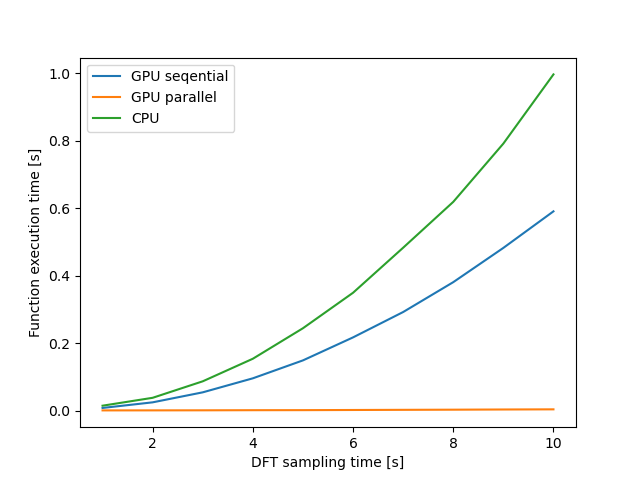
\includegraphics[width=\linewidth]{images/function_timing.png}
        \caption{Timing performance}
        \label{figure:function_timing}
    \end{minipage}
    \begin{minipage}[t]{0.45\linewidth}
        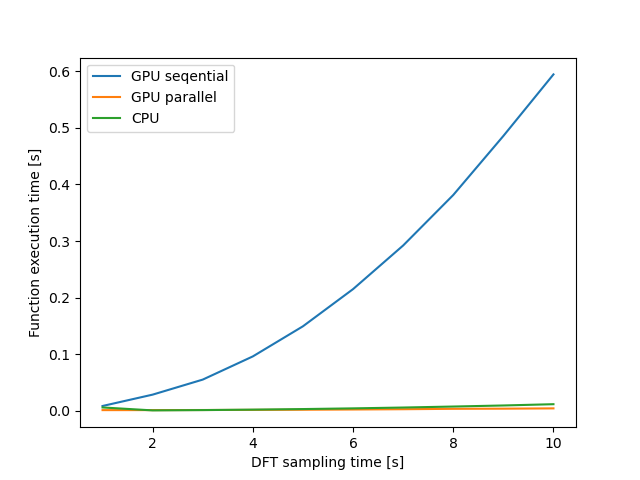
\includegraphics[width=\linewidth]{images/jit_function_timing.png}
        \caption{With @numba.jit}
        \label{figure:jit_function_timing}
    \end{minipage}
\end{figure}

\subsection{Semi parallel}
\label{subsec:semiparallel}

\section{Conclusion}
\label{sec:conclusion}

